% A0 Landscape Poster - Iran War Energy Infrastructure Analysis
% A0 dimensions: 1189mm x 841mm (landscape)
\documentclass[a0paper,landscape,25pt]{tikzposter}

% Remove default tikzposter title
\tikzposterlatexaffectionproofoff

% Color theme - light peach background
\definecolor{bgwhite}{RGB}{255,255,255}
\definecolor{lightgrey}{RGB}{240,240,240}
\definecolor{darkblue}{RGB}{25,55,95}
\definecolor{medblue}{RGB}{41,82,130}
\definecolor{lightpeach}{RGB}{255,245,230}

% Custom color theme
\definecolorstyle{CleanWhite}{
  \definecolor{colorOne}{RGB}{255,245,230}
  \definecolor{colorTwo}{RGB}{240,240,240}
  \definecolor{colorThree}{RGB}{25,55,95}
}{
  \colorlet{backgroundcolor}{colorOne}
  \colorlet{framecolor}{colorTwo}
  \colorlet{titlefgcolor}{colorThree}
  \colorlet{titlebgcolor}{colorOne}
  \colorlet{blocktitlebgcolor}{colorTwo}
  \colorlet{blocktitlefgcolor}{colorThree}
  \colorlet{blockbodybgcolor}{colorOne}
  \colorlet{blockbodyfgcolor}{black}
}

\usecolorstyle{CleanWhite}

% Minimal block style
\defineblockstyle{Minimal}{
  titlewidthscale=1, bodywidthscale=1, titlecenter,
  titleoffsetx=0pt, titleoffsety=0pt, bodyoffsetx=0pt, bodyoffsety=0pt,
  bodyverticalshift=0pt, roundedcorners=0, linewidth=0pt,
  titleinnersep=3mm, bodyinnersep=3mm
}{
  \draw[fill=blockbodybgcolor] (blockbody.south west) rectangle (blockbody.north east);
}
\useblockstyle{Minimal}

\definetitlestyle{Minimal}{
  width=\paperwidth, roundedcorners=0, linewidth=0pt, innersep=5mm,
  titletotopverticalspace=0mm, titletoblockverticalspace=5mm
}{
  \draw[fill=titlebgcolor] (\titleposleft,\titleposbottom) rectangle (\titleposright,\titlepostop);
}
\usetitlestyle{Minimal}

\usepackage{graphicx}
\usepackage{xcolor}

\title{}
\author{}
\institute{}

\begin{document}

% ===========================================================================
% TITLE BAR (~5% height = 42mm)
% ===========================================================================
\node[anchor=north west, inner sep=0pt] at (-570mm, 400mm) {
  \begin{minipage}{1140mm}
    \vspace{3mm}
    \noindent
    \begin{minipage}[c]{750mm}
      {\fontsize{60}{70}\selectfont\bfseries\color{darkblue} Energy Infrastructure at Risk: Mapping the 2026 Iran War's Impact on Gulf Oil \& Gas}\\[4mm]
      {\fontsize{30}{36}\selectfont Multi-source incident verification using OSINT, FIRMS satellite thermal anomaly detection, and geospatial infrastructure databases}
    \end{minipage}%
    \hfill%
    \begin{minipage}[c]{360mm}
      \raggedleft
      {\fontsize{26}{30}\selectfont Eric Hoffmann}\\[2mm]
      {\fontsize{22}{26}\selectfont Universit\"at Heidelberg $\cdot$ March 2026}
    \end{minipage}
    \vspace{3mm}
    \noindent\makebox[1140mm]{\color{lightgrey}\rule{1140mm}{2pt}}
  \end{minipage}
};

% ===========================================================================
% TOP ROW: Two large maps (~55% of poster height = 460mm)
% Map 1: Baseline (40% width = 456mm) | Map 2: Incident Validation (60% width = 684mm)
% Moved up to sit directly under title bar
% ===========================================================================

% MAP 1: Baseline Infrastructure (left, ~40% = 440mm width) - moved down
\node[anchor=north west, inner sep=0pt] at (-570mm, 320mm) {
  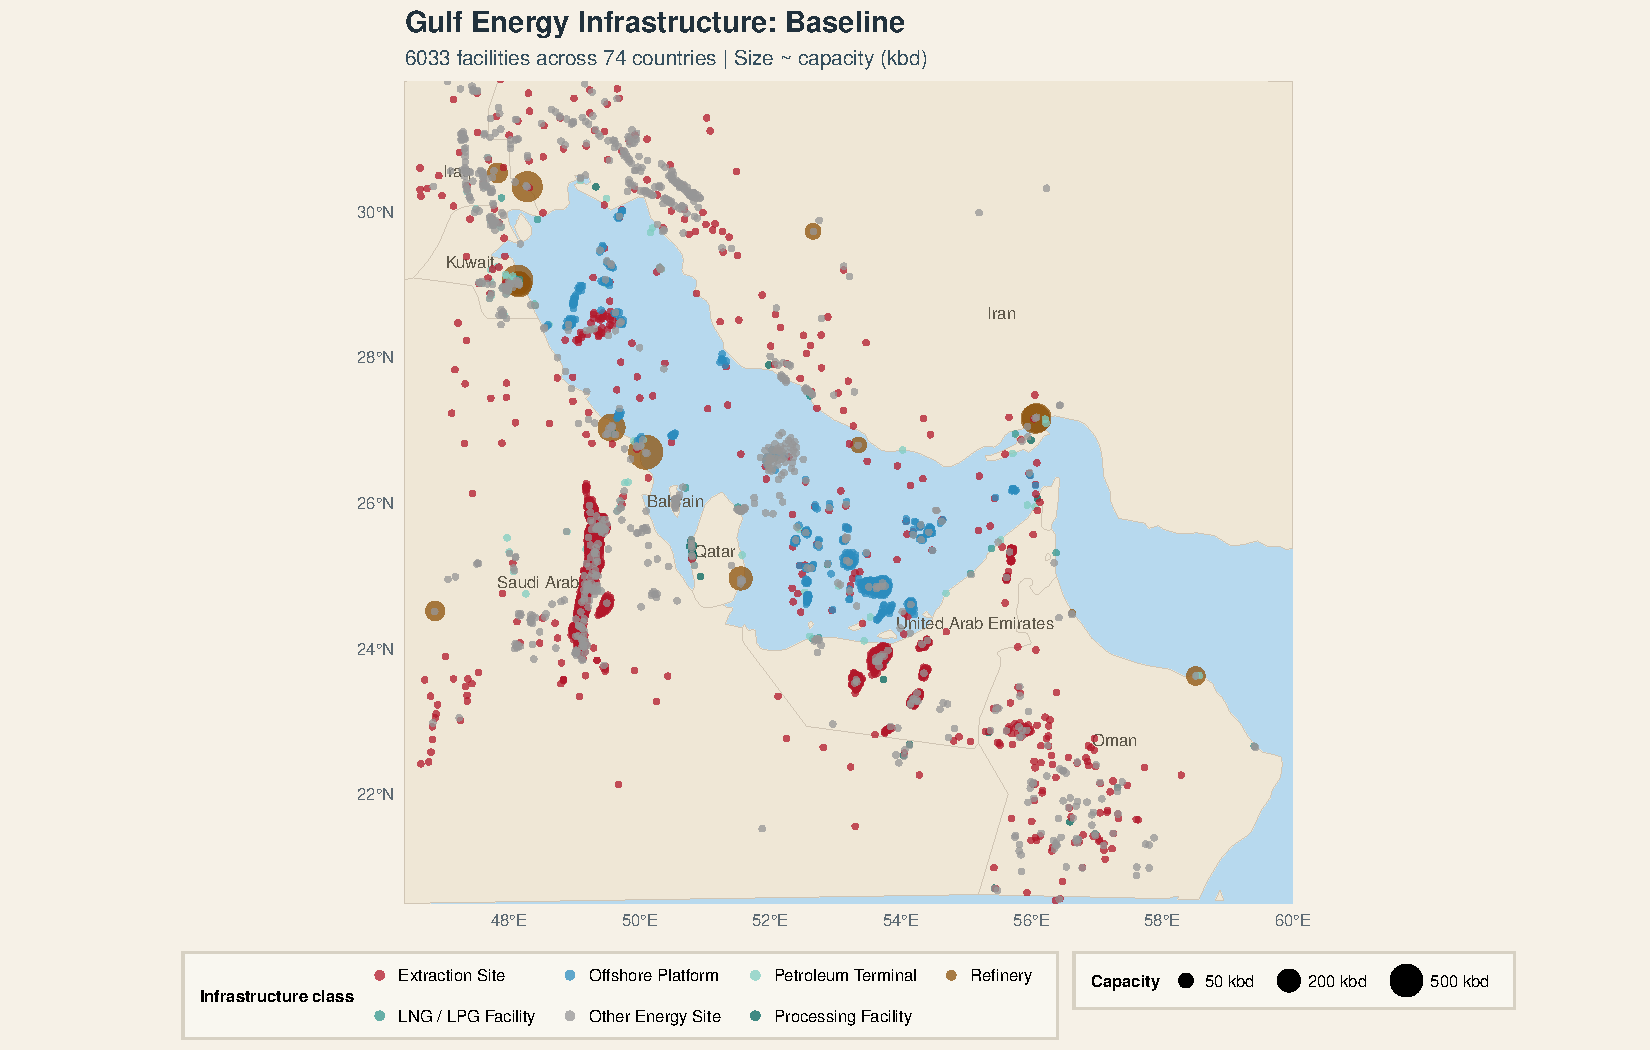
\includegraphics[width=440mm,height=400mm,keepaspectratio]{poster_graphics/infrastructure_baseline_map_01.pdf}
};

% MAP 2: Incident Validation - HERO MAP (right, positioned under title line)
\node[anchor=north east, inner sep=0pt] at (570mm, 350mm) {
  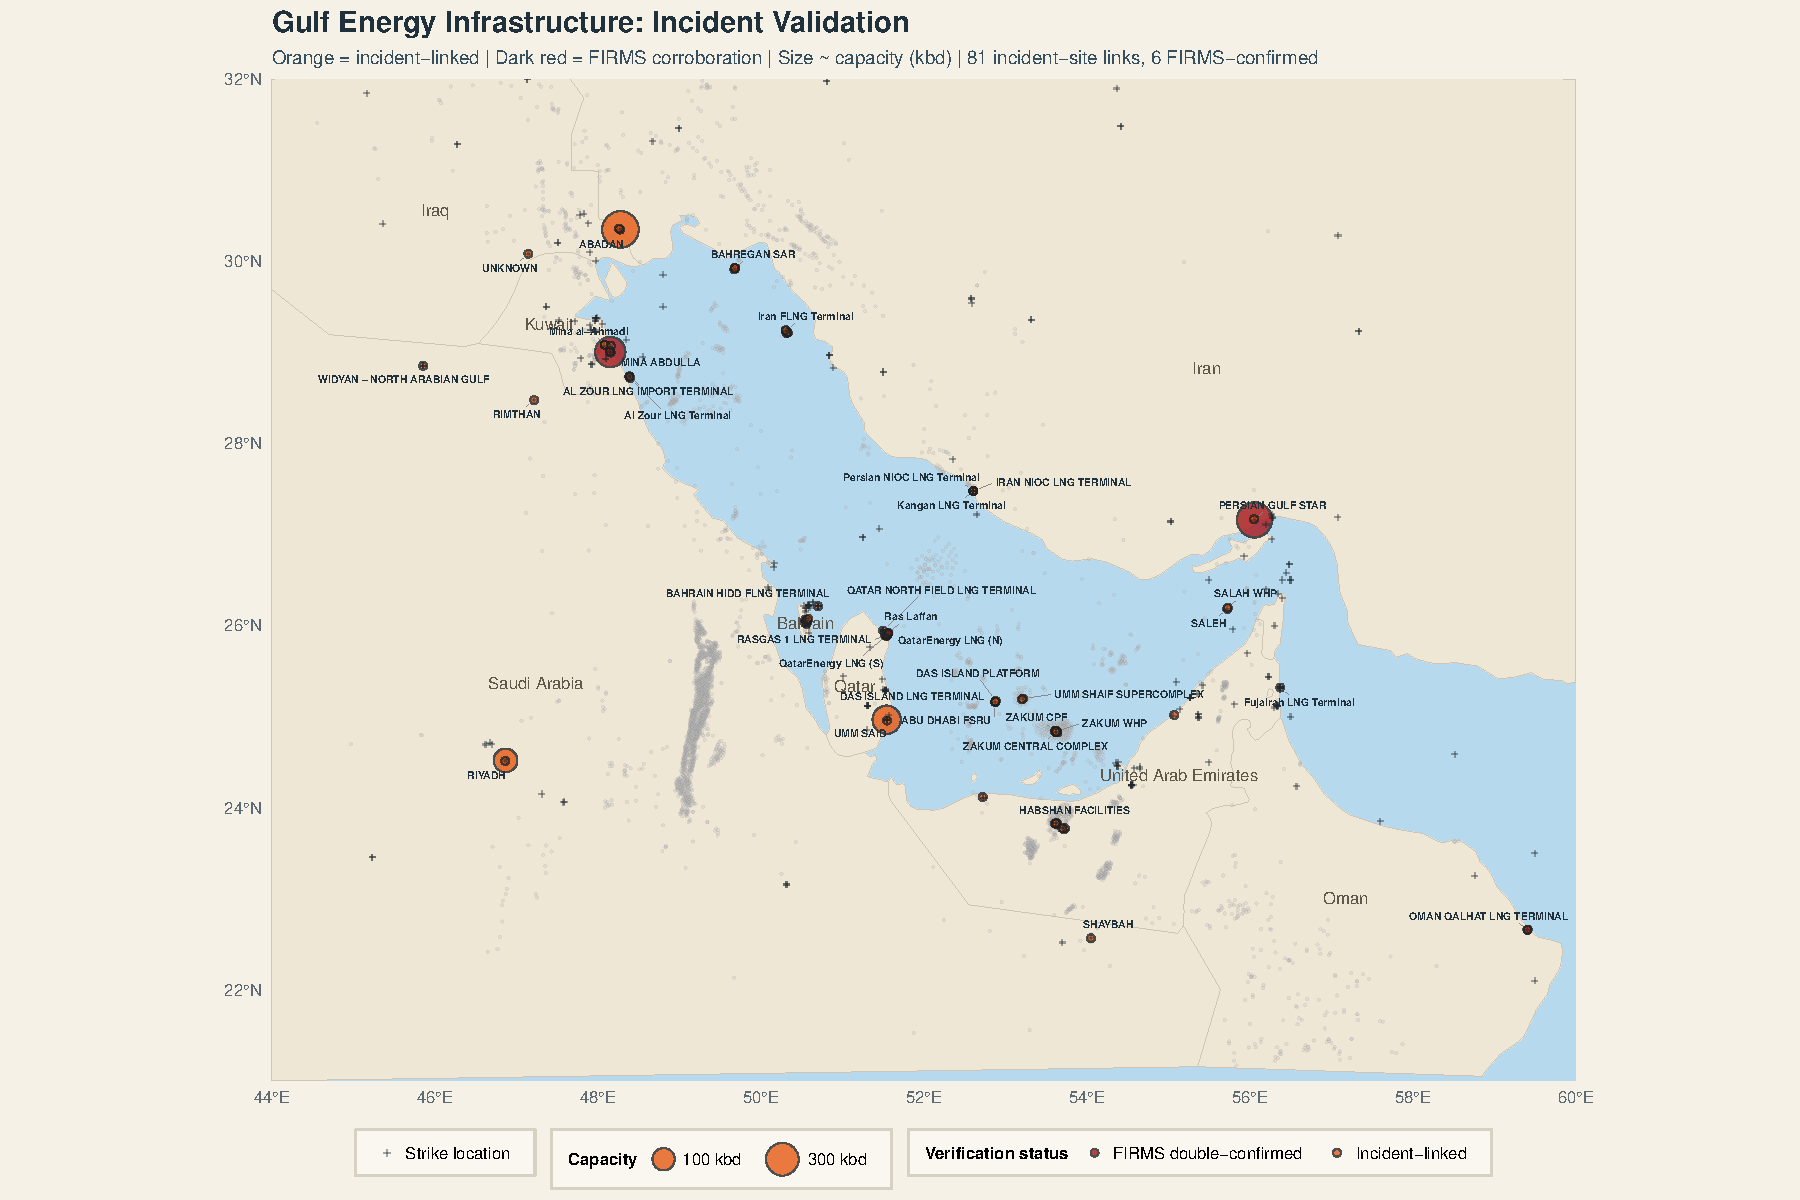
\includegraphics[width=660mm,height=430mm,keepaspectratio]{poster_graphics/incident_validation_map_10.pdf}
};

% ===========================================================================
% BOTTOM ROW: Map 3 + Chart 1 + Chart 2 (~35% height = 294mm)
% ===========================================================================

% MAP 3: Capacity at Risk - further increased size
\node[anchor=south west, inner sep=0pt] at (-570mm, -310mm) {
  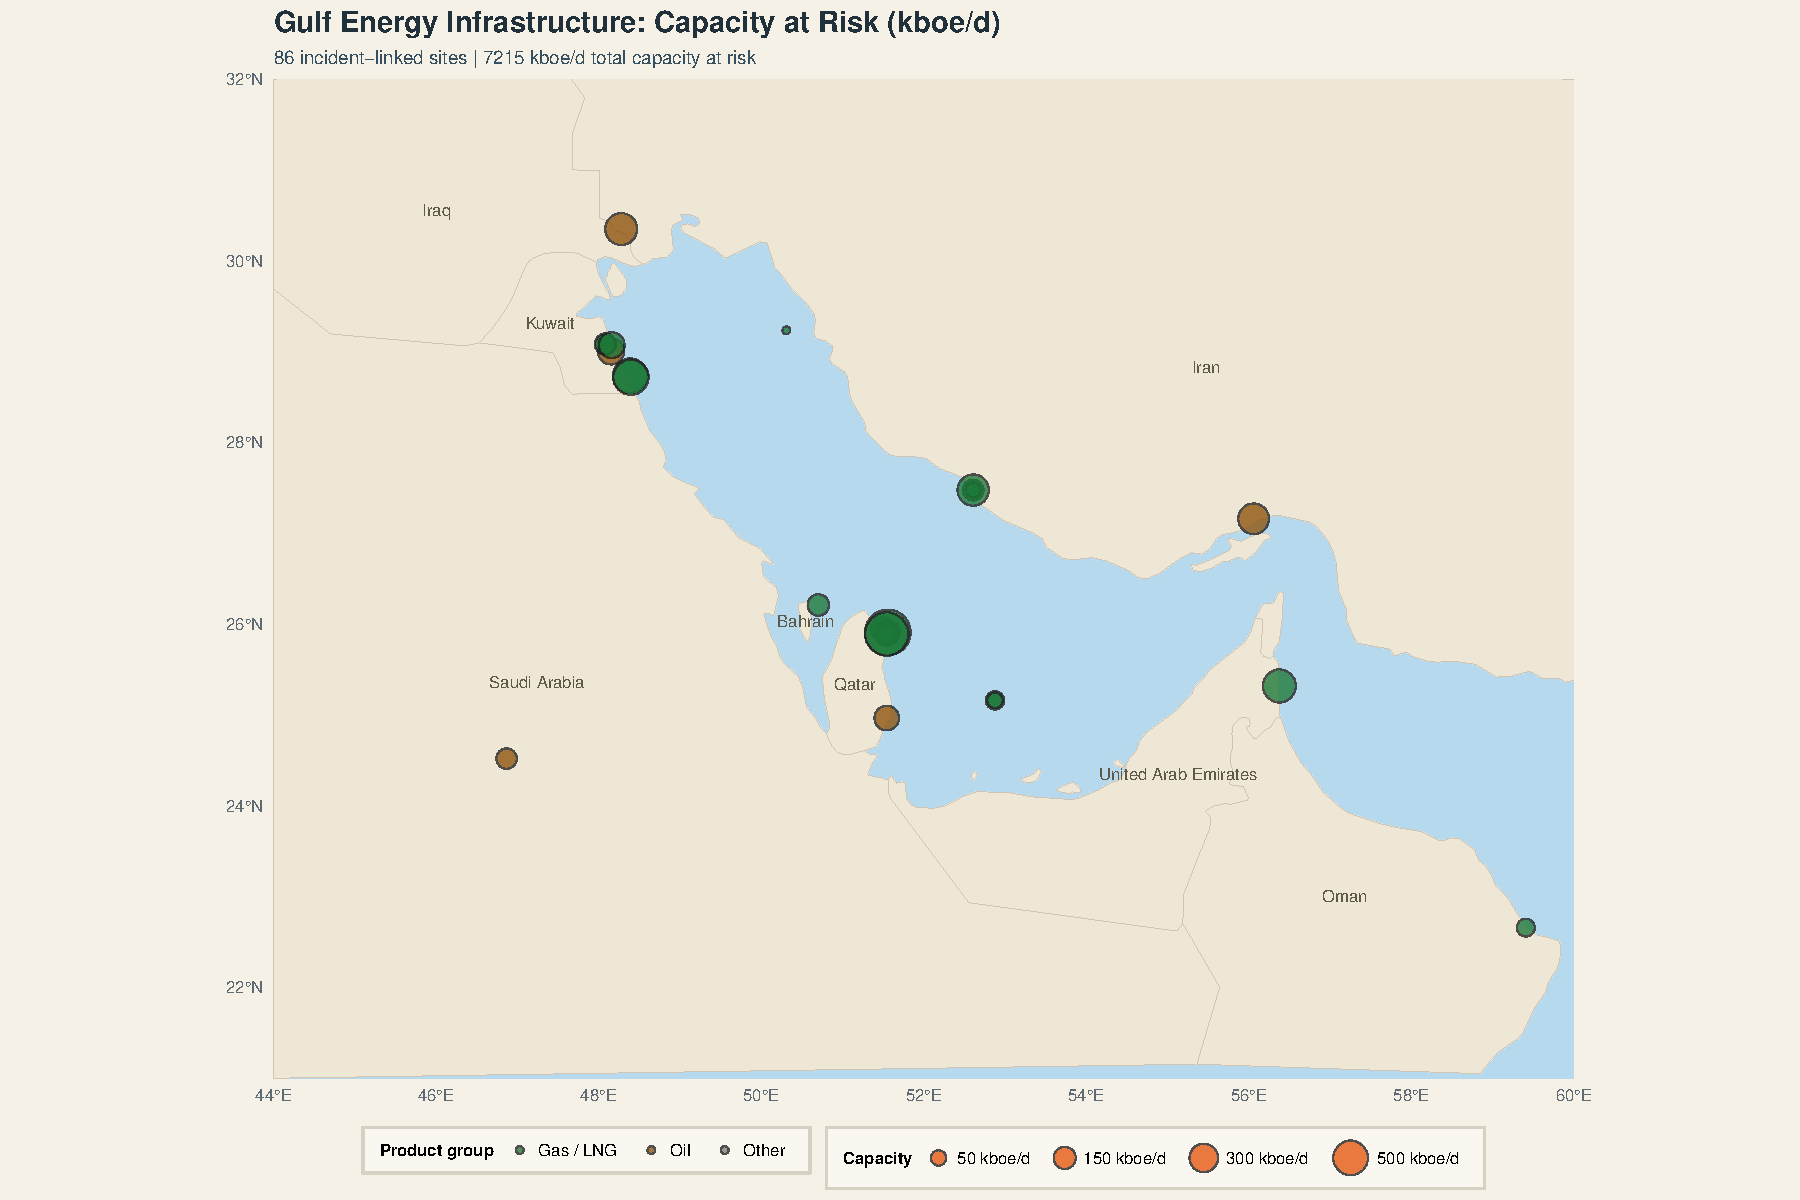
\includegraphics[width=410mm,height=310mm,keepaspectratio]{poster_graphics/capacity_at_risk_kboed_map_01.pdf}
};

% CHART 1: Country capacity bar chart (35% width = 400mm) - reduced height, moved right
\node[anchor=south, inner sep=0pt] at (-20mm, -310mm) {
  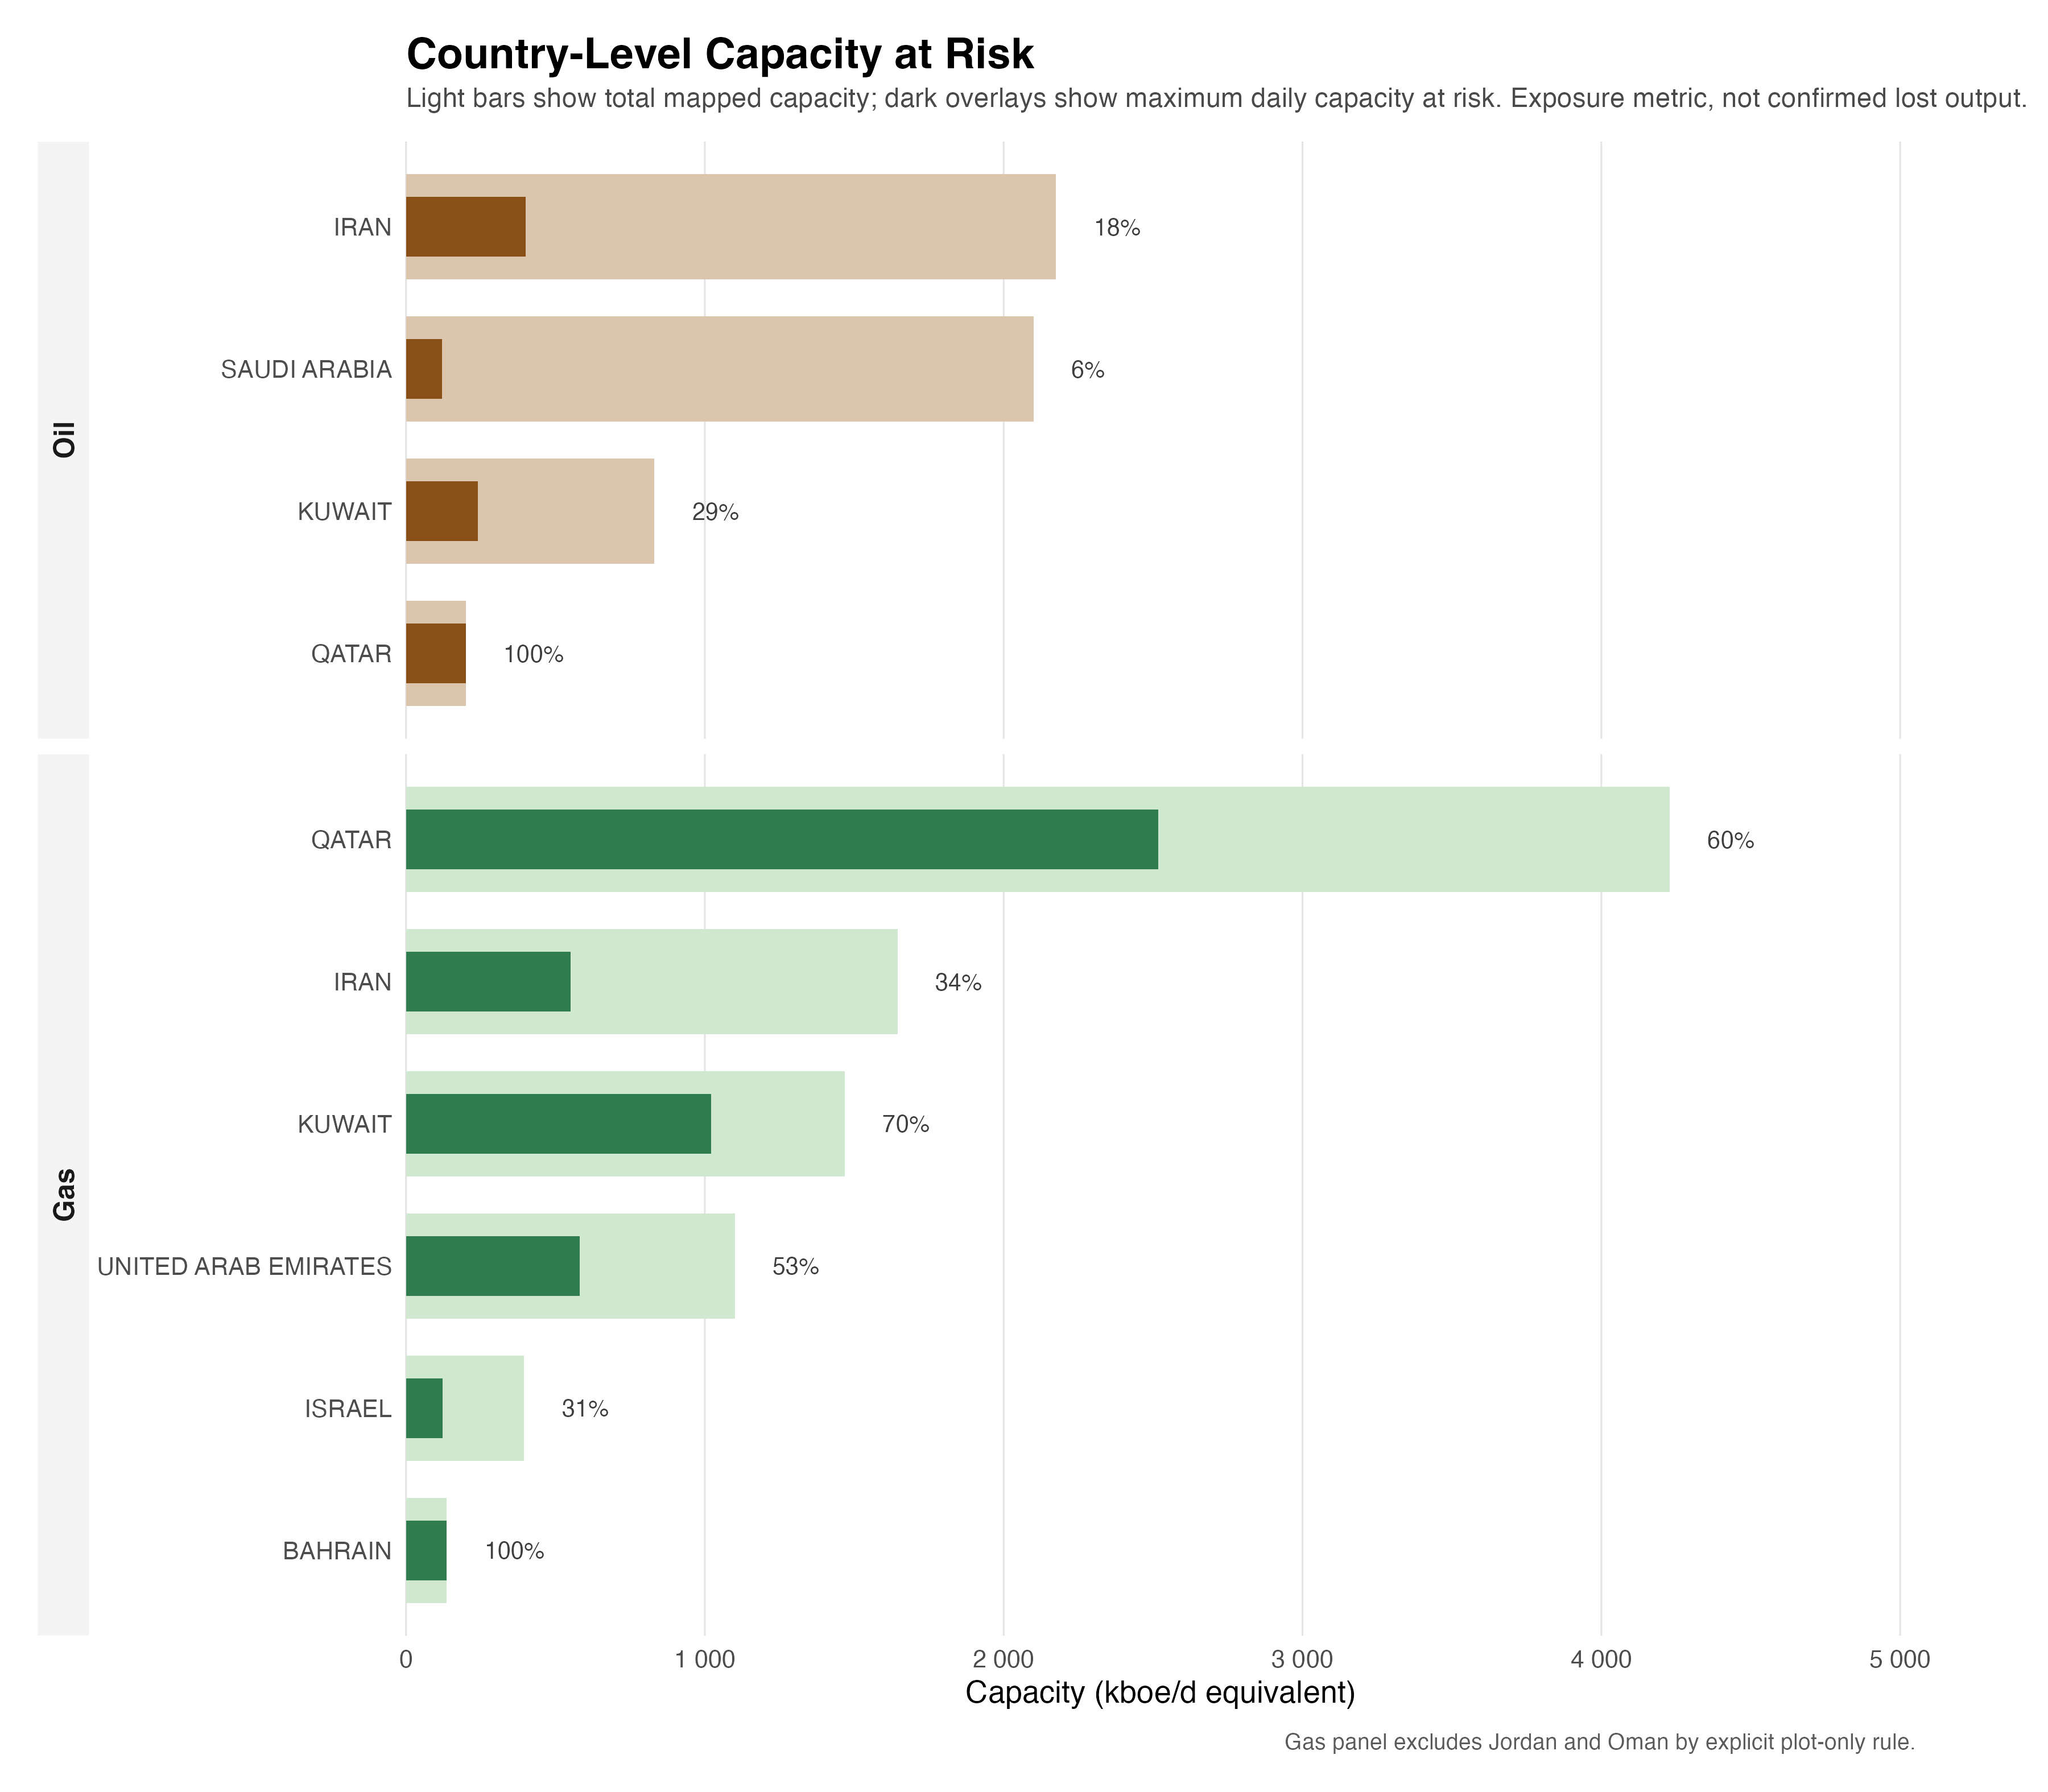
\includegraphics[width=390mm,height=230mm,keepaspectratio]{poster_graphics/fig_capacity_risk_by_country_combined_01.png}
};

% CHART 2: Daily timeline (35% width = 400mm)
\node[anchor=south east, inner sep=0pt] at (570mm, -310mm) {
  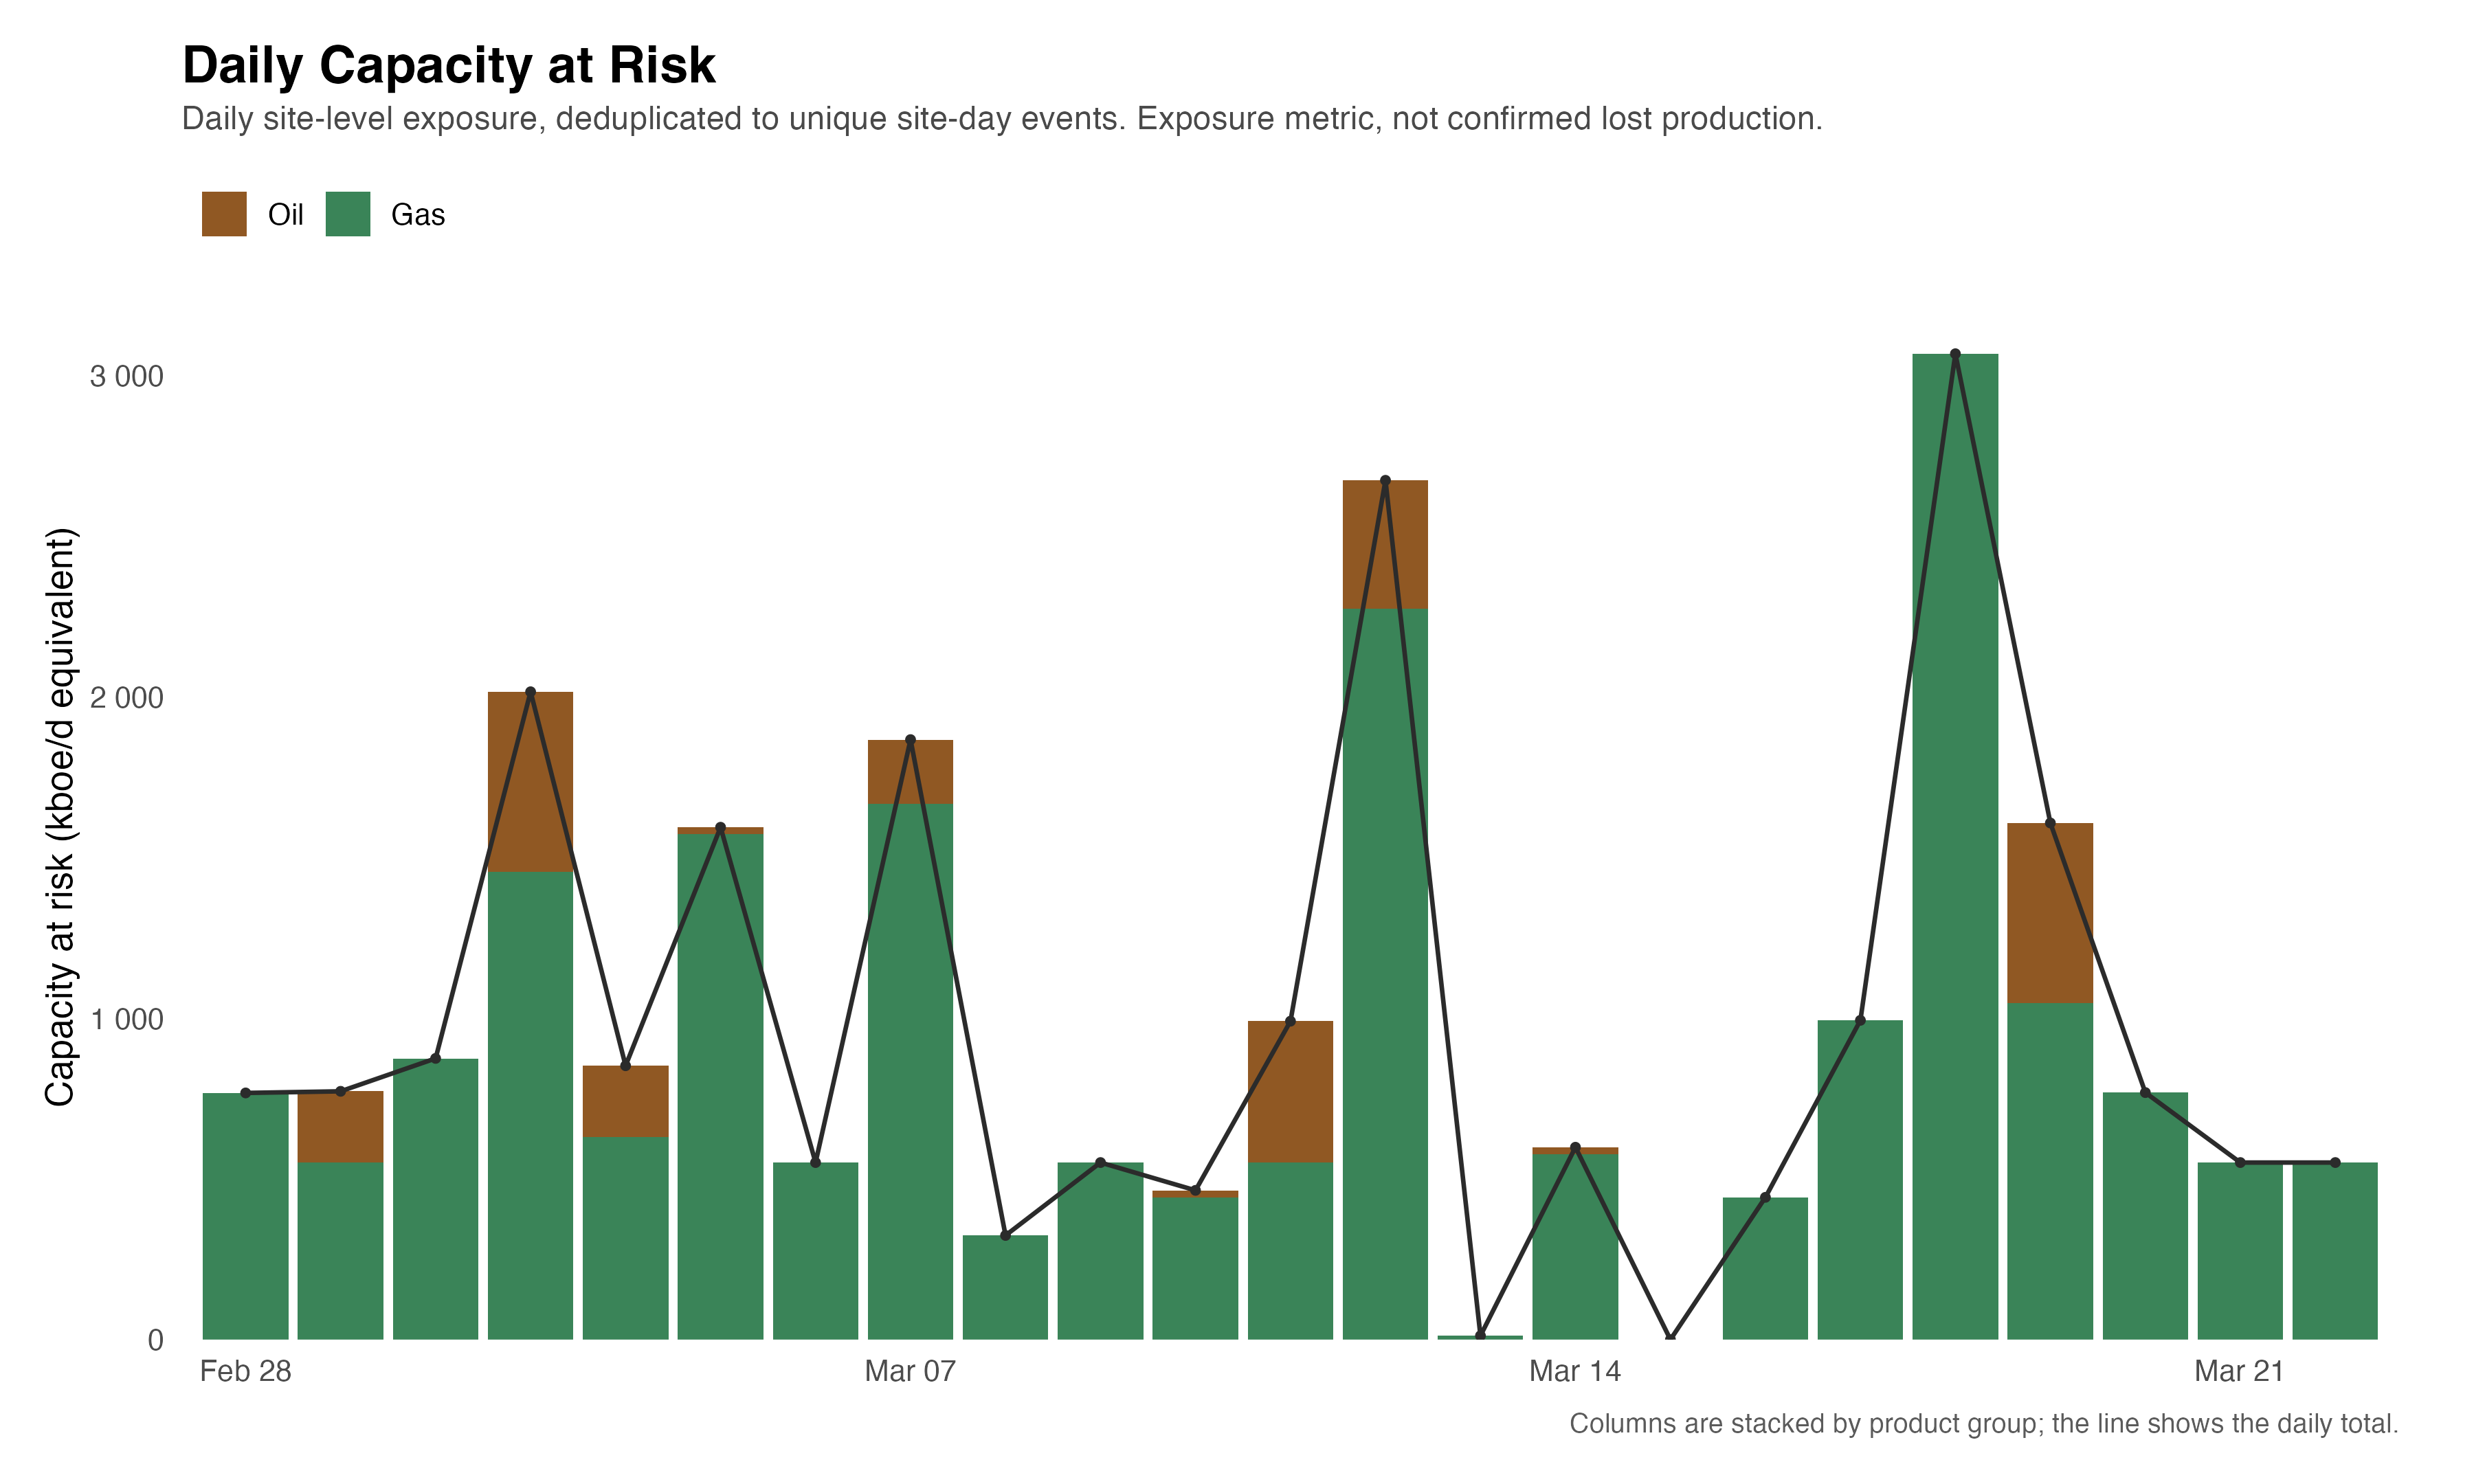
\includegraphics[width=390mm,height=260mm,keepaspectratio]{poster_graphics/fig_capacity_risk_timeseries_02.png}
};

% ===========================================================================
% METHODOLOGY STRIP (~10% height = 84mm) - Grey background bar
% ===========================================================================
\node[anchor=south, fill=lightgrey, inner sep=10mm, minimum width=1160mm, minimum height=75mm] 
  at (0mm, -400mm) {
  \begin{minipage}{1120mm}
    \begin{minipage}[t]{720mm}
      {\fontsize{22}{26}\selectfont\bfseries\color{darkblue} Methodology}\\[4mm]
      {\fontsize{16}{19}\selectfont
        The project combines geolocated strike reporting with energy infrastructure data to estimate verified exposure of Gulf hydrocarbon assets and translate that into capacity at risk. Incidents from local conflict datasets are normalized and spatially linked to mapped energy sites using a tight 2km proximity rule, while FIRMS satellite thermal anomalies are processed separately as a corroboration layer using 2km grid cells and anomaly detection against pre-conflict and historical baselines, so routine flaring is not treated as strike evidence. Verified site exposure is then joined to a canonical site-capacity base, with oil, gas, and LNG capacities harmonized into a common kboe/d equivalent metric using fixed transparent conversions. Capacity at risk is calculated conservatively by deduplicating at the unique (site\_id, incident\_day) level so the same facility is counted at most once per day, and then aggregating upward into country, product, and time-series summaries. Throughout, the measure is treated as an exposure metric, not confirmed lost production.
      }
    \end{minipage}%
    \hfill%
    \begin{minipage}[t]{190mm}
      {\fontsize{22}{26}\selectfont\bfseries\color{darkblue} Key Findings}\\[4mm]
      {\fontsize{17}{21}\selectfont
        \textbf{86} incident-linked energy facilities\\
        \textbf{7,215 kboe/d} capacity at risk\\
        \textbf{6} FIRMS-confirmed strikes\\
        Largest: Ras Laffan LNG, $\sim$1,400 kboe/d
      }
    \end{minipage}%
    \hfill%
    \begin{minipage}[t]{170mm}
      {\fontsize{22}{26}\selectfont\bfseries\color{darkblue} Data Sources}\\[4mm]
      {\fontsize{15}{19}\selectfont
        For full bibliography, see:\\[2mm]
        \texttt{github.com/Grumpylenard/}\\
        \texttt{Iran\_EF-TP4\_2026\_DS4E}
      }
    \end{minipage}
  \end{minipage}
};

\end{document}